% =====================================================================
% When Does Hyperparameter-Free Decoding Break?
% A Rényi-alpha Analysis of Entropy-Threshold Sampling for Code & Reasoning
%
% CONTENT DRAFT (Narrative A). Every number traces to:
%   docs/research/paperA_master_numbers.md      (APPS + MBPP + HumanEval)
%   docs/research/paperA_renyi_nonequivalence.md (alpha family)
%   docs/research/paperA_loop_positioning.md     (reasoning loops)
%   paper/draft.md + paper/sources.md            (MBPP/HE spine)
%
% Uses the generic `article` class so it compiles anywhere (incl. Overleaf).
% To submit to ICLR 2027: download iclr2027_conference.sty from the ICLR site,
% replace the documentclass/preamble block marked [ICLR-SWAP] below, and set
% the paper to double-blind (author block already anonymized).
% =====================================================================
\documentclass[11pt]{article}                       % [ICLR-SWAP]
\usepackage[margin=1in]{geometry}                    % [ICLR-SWAP: remove; iclr sty sets layout]
\usepackage[utf8]{inputenc}
\usepackage{amsmath,amssymb}
\usepackage{booktabs}
\usepackage{graphicx}
\usepackage{subcaption}
\usepackage{multirow}
\usepackage[numbers]{natbib}
\usepackage[hidelinks]{hyperref}
\usepackage{xcolor}
\newcommand{\td}[1]{\textcolor{red}{[TODO: #1]}}     % visible authoring notes
\newcommand{\tsum}{\ensuremath{\textstyle\sum}}
\graphicspath{{figures/}}

\title{When Does Hyperparameter-Free Decoding Break?\\
A R\'enyi-$\alpha$ Analysis of Entropy-Threshold Sampling\\ for Code and Reasoning}
\author{Anonymous authors\\ \textit{Paper under double-blind review}}
\date{}

\begin{document}
\maketitle

\begin{abstract}
Hyperparameter-free decoders promise to remove temperature and top-$p$ tuning by deriving a
truncation threshold directly from the token distribution. We ask \emph{when} that promise holds for
code generation. Across 13 model checkpoints on MBPP-500 and HumanEval-164, and two reasoning models
on APPS competitive-programming problems, we find a sharp boundary. p-less sampling
(threshold $\tsum_i p_i^2$) behaves as a \emph{high-accuracy, low-diversity} decoder: it is
competitive---occasionally best---at pass@1 on short base-model completions, but is dominated at
pass@10 by temperature, and \emph{silently degenerates} on long chain-of-thought, where peaked
next-token distributions raise the threshold until only the mode survives, driving 15--42\% of
reasoning traces into non-terminating loops. We trace both failures to a single mechanism---the
interaction of distribution peakedness with hard thresholding---and study the R\'enyi-$\alpha$ family
$\tau_\alpha(p)=\tsum_i p_i^\alpha$ ($\alpha=2$ recovers p-less) as a diagnostic knob, a
generalization the method's origin paper proposes but never evaluates beyond $\alpha=2$. Raising
$\alpha$ flattens the survivor set, monotonically eliminates looping (truncation $42\%\!\to\!0.3\%$),
and recovers most lost accuracy, \emph{but does not surpass well-tuned temperature sampling} on either
reasoning model. Our contribution is thus a characterization of \emph{when} parameter-free decoding
helps and when it breaks, the first empirical $\alpha$-sweep of entropy-threshold decoding, and a
reproducibility analysis showing how tokenizer- and numerics-level bugs can fabricate apparent
decoding-method effects of up to 22\,pp.
\end{abstract}

\section{Introduction}\label{sec:intro}
Code generation with large language models has converged on a small set of decoding policies---greedy
or beam search at deployment, temperature sampling at evaluation---and a tradition of treating
decoding as an afterthought. The benchmarks encourage this: pass@1 rewards a single confident guess,
pass@10 rewards diversity, and few systems agree on which to optimize.

Standard truncation samplers introduce hyperparameters that interact non-obviously with model
peakedness. Top-$p$~\citep{holtzman2020curious}, top-$k$, $\eta$-sampling~\citep{hewitt2022truncation},
min-$p$~\citep{nguyen2024minp}, and top-$n\sigma$~\citep{tang2024topnsigma} each carry one or two free
parameters whose right setting depends on the model, the task, and the desired
correctness/diversity trade-off. \citet{shi2024decoding} document wide sensitivity to these knobs
across decoding methods on Llama-2-7B over MBPP and HumanEval, but do not consider
hyperparameter-free alternatives. \citet{tan2025pless} propose \textbf{p-less} and
\textbf{p-less-norm}: truncation samplers whose admission threshold is computed from the
distribution's collision entropy, with no tunable knobs. The proposal is appealing, but the original
work evaluates only on math, reasoning, and creative writing---not code, where outputs are
syntactically constrained and probability mass is often concentrated on a single correct token.

We provide the first systematic evaluation of p-less on code, and find that its behavior is governed
by a single property---\emph{distribution peakedness}---that predicts both where it helps and where
it silently fails. Our contributions:
\begin{enumerate}\itemsep2pt
  \item \textbf{A when-does-it-help boundary} (\S\ref{sec:helps}): across 13 checkpoints on MBPP/HE
    and two reasoning models on APPS, p-less is competitive at pass@1 but dominated at pass@10, and
    catastrophic on long chain-of-thought.
  \item \textbf{A mechanism} (\S\ref{sec:breaks}): peakedness $\times$ hard threshold collapses the
    survivor set to the mode, producing the pass@10 diversity gap and the reasoning loop as two faces
    of the same effect.
  \item \textbf{The first empirical $\alpha$-sweep} of an entropy-threshold sampler
    (\S\ref{sec:alpha}), with a self-contained non-equivalence to the origin paper's un-evaluated
    R\'enyi form.
  \item \textbf{Code-specific reasoning-loop findings} (\S\ref{sec:breaks}): a paraphrastic-vs-verbatim
    loop breakdown on APPS, and a verified non-transfer of a published hidden-state loop precursor to
    code.
  \item \textbf{A reproducibility post-mortem} (\S\ref{sec:repro}): three silent pipeline bugs shifted
    pass@1 by up to 22\,pp and fabricated a decoding-method result that reversed once fixed.
\end{enumerate}
The headline is conditional, not promotional: \textbf{p-less is a calibration-free default that is
useful where distributions are flat and silently broken where they are peaked}; the value it delivers
is the removed hyperparameter, not raw pass@k uplift.

\section{Background and Related Work}\label{sec:bg}
\paragraph{p-less and p-less-norm.} Given a distribution $p$ over a vocabulary of size $v$, p-less
sets its threshold to the collision entropy $\tau_{\text{pless}}=\tsum_i p_i^2$ and admits tokens with
$p_i \ge \tau_{\text{pless}}$; p-less-norm relaxes this to
$\tau_{\text{norm}}=(v\tsum_i p_i^2 - 1)/(v-1)$, admitting more tail tokens~\citep{tan2025pless}.
Survivors are renormalized and sampled; neither takes a top-$k$, top-$p$, or $\eta$ budget---only an
optional pre-truncation temperature.

\paragraph{Decoding on code.} \citet{shi2024decoding} benchmark a wide panel (greedy, beam, top-$p$,
top-$k$, $\eta$/typical, FSD, contrastive, Mirostat, temperature) on Llama-2-7B over MBPP and
HumanEval; their analysis predates p-less. We use their published Llama-2-7B MBPP numbers as an
external comparison in \S\ref{sec:helps}. \citet{holtzman2020curious} established that
likelihood-maximizing decoding collapses toward the mode and produces repetitive degeneration---the
mechanism our peaked-distribution failure instantiates.

\paragraph{Reasoning loops.} Recent work characterizes non-terminating loops in reasoning models.
\citet{duan2026circular} show loops are often semantically redundant while lexically distinct and
predict them from hidden-state transitions; \citet{xie2025wordsalad} note that reasoning models
``typically do not exhibit strictly verbatim repetitions'' and catch the resulting ``word salad''
with a hidden-state probe; \citet{pipis2025loop} show reasoning models loop at low temperature.
Crucially, \emph{all of this work is on math/QA and is detection-focused}: none evaluates on code,
none reports the fraction of loops that are paraphrastic, and none studies a truncation sampler as a
\emph{cause} or \emph{preventive} of looping (\S\ref{sec:breaks} closes these gaps).
\citet{yang2025recover} show models identify but fail to recover from unhelpful thoughts, with
inverse scaling; \citet{yang2025deer} and \citet{muennighoff2025s1} control reasoning length
reactively (early exit) or by budget forcing.

\section{Methodology}\label{sec:method}
\paragraph{Models and benchmarks.} We evaluate 13 checkpoints (Meta Llama-2 base/chat, Code
Llama~\citep{roziere2023codellama} base/instruct, Mistral Codestral, Qwen2.5-Coder~\citep{hui2024qwen25coder}
and Qwen3-Coder; 1.3B--30B) on MBPP-500~\citep{austin2021mbpp} and HumanEval-164~\citep{chen2021humaneval}.
For the reasoning regime we use DeepSeek-R1-Distill-Llama-8B~\citep{deepseekai2025r1} and
Qwen3-8B~\citep{yang2025qwen3} on 252 APPS ``interview'' problems with the thinking phase enabled.
Instruct models use \texttt{apply\_chat\_template}; base models use bare-prompt tokenization.

\paragraph{Sampling and metrics.} Stochastic configurations draw 10 samples/task. We report pass@$k$
with the unbiased estimator of \citet{chen2021humaneval}, cover@$t$ (fraction of tasks with
$\ge\!\lceil t\cdot n\rceil$ correct samples), structural diversity (mean pairwise Zhang--Shasha tree
edit distance~\citep{zhang1989simple} over correct samples), and CodeBLEU-based
diversity~\citep{ren2020codebleu}. For APPS we additionally report the non-termination
(truncation) rate: the fraction of samples that never close the thinking phase within the token
budget---our loop proxy. Per-task binomial SE is $\approx 1.75$\,pp on MBPP-500 and $\approx 2.8$\,pp
on HumanEval-164; differences below $\sim$2\,SE are reported as directional.

\paragraph{The R\'enyi-$\alpha$ family.} We study $\tau_\alpha(p)=\tsum_i p_i^\alpha$ with
$\alpha \ge 2$; $\alpha=2$ is exactly p-less. \S\ref{sec:alpha} relates this to the origin paper's
proposal.

\section{Where p-less helps: flat distributions}\label{sec:helps}
On \emph{weaker base models}, where the model is uncertain at most steps, p-less admits a small
tractable survivor set and is competitive at pass@1. On Llama-2-7B (MBPP-500), merged with the
decoding methods surveyed by \citet{shi2024decoding}, p-less-norm at $T{=}0.6$ is the top-ranked
sampler (Table~\ref{tab:mbpp}), ahead of FSD-d and beam-8; plain temperature ranks 15/19.

\begin{table}[t]\centering
\caption{MBPP-500 pass@1 on Llama-2-7B (base), our p-less variants merged with the
\citet{shi2024decoding} survey (rank out of 19). Source: \texttt{comparison\_report.md}.}
\label{tab:mbpp}
\begin{tabular}{lcc}
\toprule
Method & pass@1 (\%) & Rank \\
\midrule
p-less-norm ($T{=}0.6$) & 22.3 & \textbf{1} \\
p-less ($T{=}0.6$)      & 22.2 & 2 \\
p-less ($T{=}1.0$)      & 19.8 & 4 \\
p-less-norm ($T{=}1.0$) & 19.1 & 7 \\
temperature ($T{=}0.7$) & 13.2 & 15 \\
\bottomrule
\end{tabular}
\end{table}

But the pass@1 win comes with a diversity deficit. Table~\ref{tab:he} shows the recurring
\textbf{pass@1-vs-pass@10 trade-off} on HumanEval: p-less matches or beats greedy and temperature at
pass@1 (Codestral 78.0 vs.\ 72.6; Qwen2.5-Coder-7B-Instruct 87.5 vs.\ greedy 84.1) but is dominated at
pass@10, where temperature/top-$p$ cover more distinct solutions (CodeLlama 62.8 vs.\ 38.4). p-less
occupies the high-pass@1, low-diversity corner of the Pareto frontier (Fig.~\ref{fig:pareto}); it
sits \emph{on} each model's frontier but does not extend it, because the threshold prunes more
aggressively than temperature once mass concentrates.

\begin{table}[t]\centering
\caption{HumanEval-164 pass@1$\to$pass@10 (\%): the accuracy--diversity trade-off. p-less is best/tied
at pass@1, dominated at pass@10. Source: \texttt{full\_precision\_results/analysis/report.md}.}
\label{tab:he}
\begin{tabular}{lccc}
\toprule
Model & p-less (best) & temp/top-$p$ (best) & greedy \\
\midrule
CodeLlama-7B-Instruct        & 36.1 $\to$ 38.4 & 36.2 $\to$ \textbf{62.8} & 36.0 \\
Codestral-22B                & \textbf{78.0} $\to$ 84.8 & 72.6 $\to$ \textbf{91.5} & 75.6 \\
Qwen2.5-Coder-7B-Instruct    & \textbf{87.5} $\to$ 87.8 & 79.0 $\to$ \textbf{94.5} & 84.1 \\
Qwen3-Coder-30B-A3B-Instruct & 78.9 $\to$ 79.9 & 76.2 $\to$ \textbf{86.6} & 75.6 \\
\bottomrule
\end{tabular}
\end{table}

\begin{figure}[t]\centering
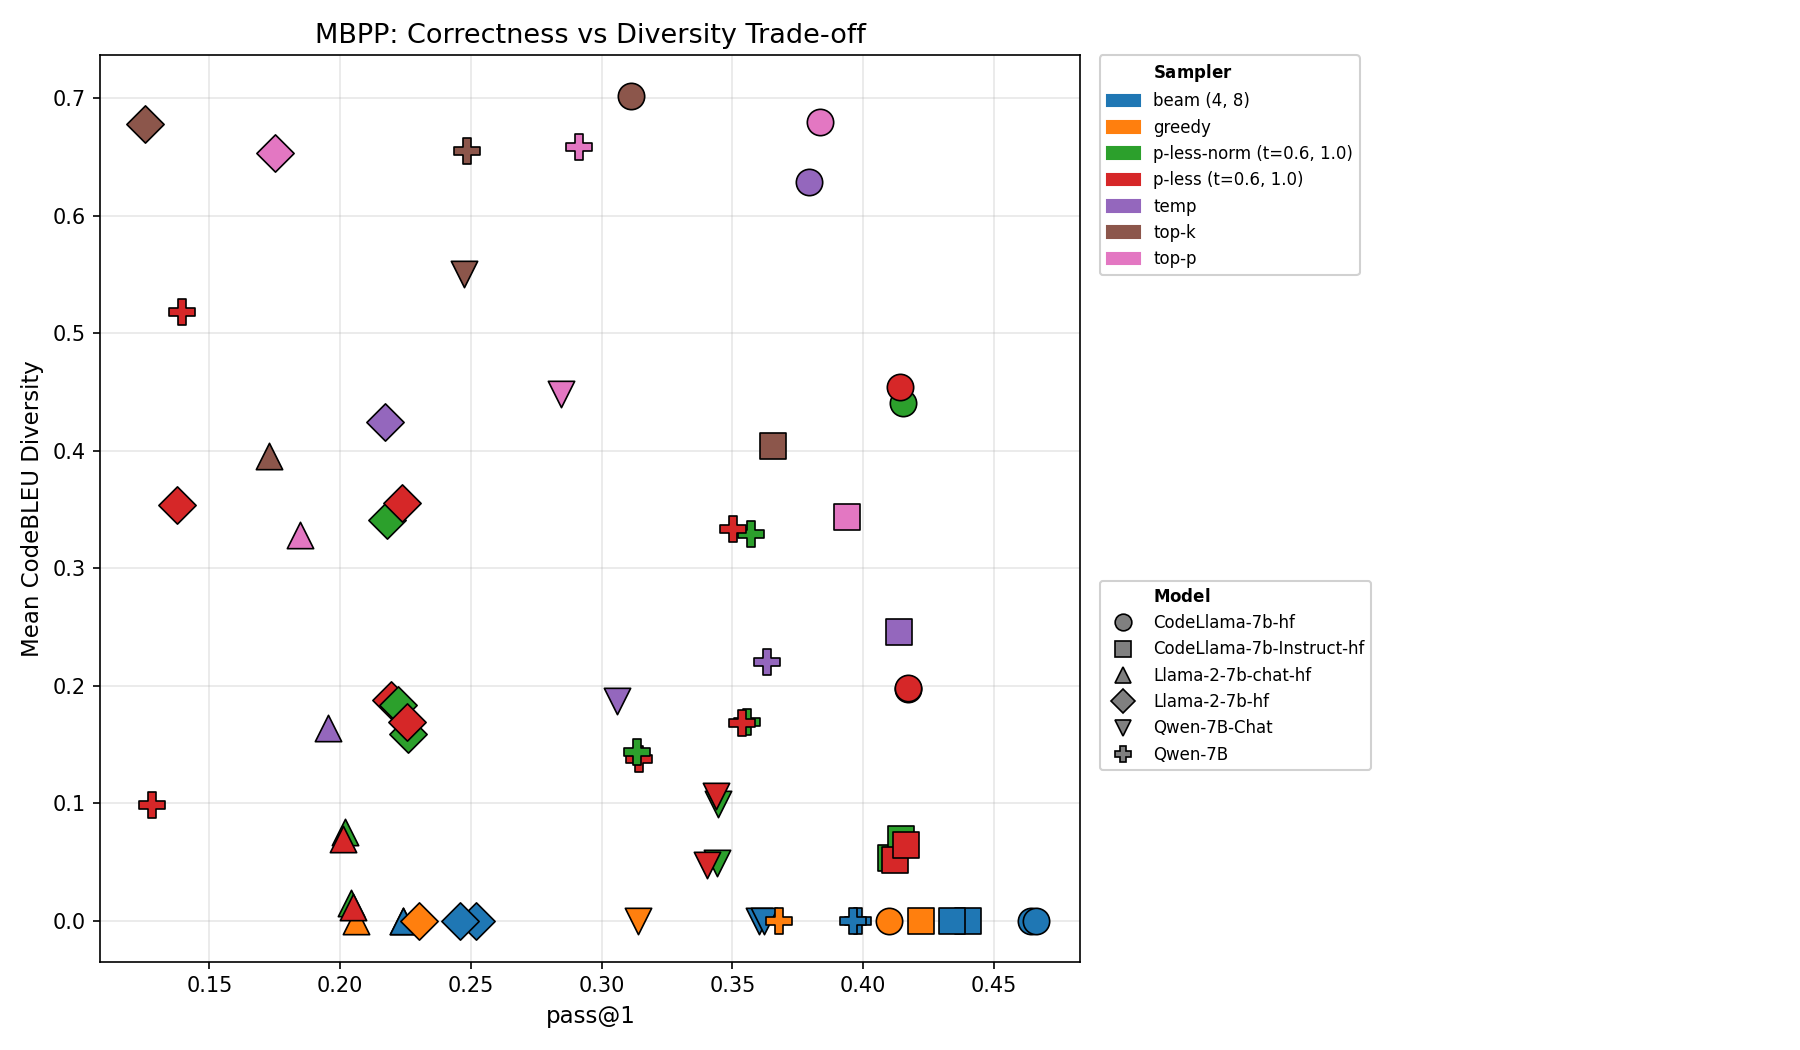
\includegraphics[width=0.68\linewidth]{fig_pareto.png}
\caption{Pass@1 vs.\ structural diversity on MBPP-500 (base/chat models). p-less/p-less-norm occupy
the high-pass@1/low-diversity corner; temperature reaches diversities no p-less setting reproduces in
the safe range. \td{regenerate at final DPI; confirm legend readable at column width}}
\label{fig:pareto}
\end{figure}

\section{Where p-less breaks: peaked distributions and long CoT}\label{sec:breaks}
\paragraph{The temperature cliff.} As pre-truncation temperature rises, p-less does not gracefully
diversify---it collapses. On a six-point HumanEval sweep (Fig.~\ref{fig:tempsweep}), pass@1 is flat in
$T\!\in\![0.7,1.5]$ but every temperature-sensitive model falls off a cliff by $T\!=\!2.5$. On the
most peaked model (Qwen3-Coder-30B) p-less is $T$-immune because the threshold admits only the top
token at every $T$---p-less has degenerated to greedy.

\begin{figure}[t]\centering
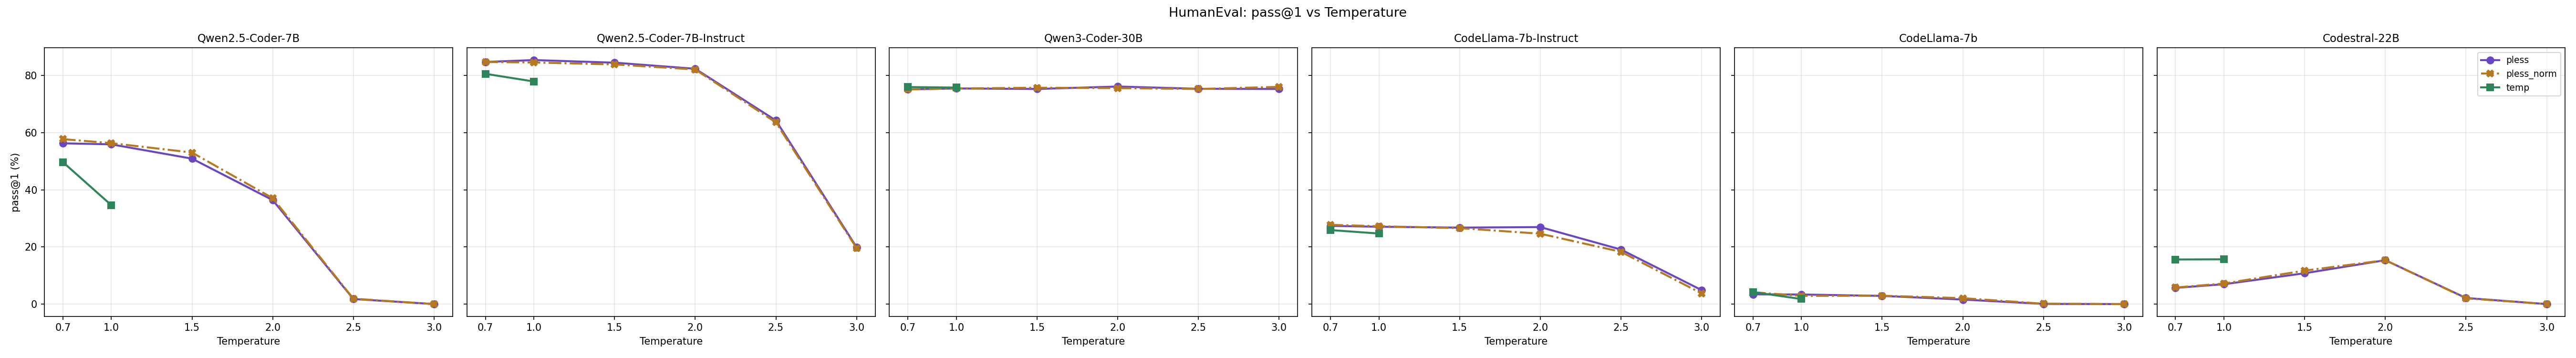
\includegraphics[width=0.62\linewidth]{fig_temp_sweep.png}
\caption{Pass@1 vs.\ pre-truncation temperature on HumanEval-164 (p-less, six models): a sweet spot at
$T\!\in\![0.7,1.5]$ and a cliff by $T\!=\!2.5$.}
\label{fig:tempsweep}
\end{figure}

\paragraph{Long chain-of-thought: silent loops.} The peakedness pathology is most damaging on
reasoning models, whose thinking phase is long and low-entropy. With default p-less ($\alpha=2$),
\textbf{41.8\% of DeepSeek-R1-Distill and 14.5\% of Qwen3-8B APPS traces never terminate}---they loop
until the token cap---and pass@1 is the worst of any decoder we test (DeepSeek 0.392, Table~\ref{tab:apps}).
The mechanism is the same as the pass@10 gap: on a near-deterministic step the collision-entropy
threshold approaches the top probability, so the survivor set collapses to the mode and the model
re-derives the same continuation. This inverts the usual view of truncation as a cure for
repetition~\citep{holtzman2020curious}: a threshold tied to $\tsum_i p_i^2$ \emph{amplifies} looping
exactly where the model is confident.

\paragraph{What the loops look like on code.} Prior loop studies are math/QA-only and detection-focused
\citep{duan2026circular,xie2025wordsalad}. Categorizing all non-terminating APPS traces, only
$\sim$41--50\% are \emph{verbatim} statement loops (Qwen3-8B 40.7\%, DeepSeek 49.8\%); a comparable
share---41.3\% (Qwen3-8B) and 46.8\% (DeepSeek)---are \emph{paraphrastic}: the model re-explores the
same idea in drifting words (best periodicity self-match median $0.23$--$0.26$; 73--74\% of these
traces below $0.5$), so no token recurs and the loop is invisible to verbatim $n$-gram detection.
Neither prior paper reports this breakdown. Consistent with it, a published hidden-state loop
precursor~\citep{duan2026circular} \emph{does not transfer}: reimplementing its probe+CUSUM detector on
Qwen3-8B code traces catches only $\sim$17--20\% of terminal loops before onset (vs.\ the
$0.64$--$0.76$ it reports on synthetic \emph{verbatim} loops), and its ``semantic-precedes-textual''
precursor is absent before onset (pre-onset periodicity at or below chance). Because paraphrastic loops
lack the clean textual onset the precursor assumes, these rates are directional rather than a strict
numerical comparison; the robust, qualitative finding is that paraphrastic code loops offer no
precursor gap to exploit.

\section{The $\alpha$ knob: a diagnostic lens, not a new SOTA sampler}\label{sec:alpha}
\paragraph{Raising $\alpha$ removes the loop.} The R\'enyi family $\tau_\alpha=\tsum_i p_i^\alpha$
flattens the survivor set as $\alpha$ grows. On APPS (Fig.~\ref{fig:appsalpha}, Table~\ref{tab:apps}),
raising $\alpha$ from 2 to 5 collapses truncation ($41.8\%\!\to\!0.3\%$ DeepSeek; $14.5\%\!\to\!0.6\%$
Qwen) and recovers most of the lost pass@1 ($0.392\!\to\!0.483$; $0.625\!\to\!0.686$), monotonically
and with no per-task tuning.

\begin{table}[t]\centering
\caption{APPS (252 tasks, $n{=}10$, thinking on): pass@1 / pass@10 / non-termination \%. Raising
$\alpha$ removes loops and recovers accuracy, but the best $\alpha$ only \emph{ties} well-tuned
temperature. Regenerated live via \texttt{build\_decoder\_comparison\_table.py}
(pass@$k$ cross-verified vs.\ stored).}
\label{tab:apps}
\begin{tabular}{lccc}
\toprule
Config & pass@1 & pass@10 & non-term.\ \% \\
\midrule
\multicolumn{4}{l}{\textit{DeepSeek-R1-Distill-Llama-8B}}\\
p-less $\alpha{=}5$          & 0.483 & 0.714 & 0.3 \\
temp $T{=}1.0$, $p{=}0.95$   & 0.480 & \textbf{0.726} & 0.0 \\
p-less $\alpha{=}4$          & 0.473 & 0.710 & 1.4 \\
adaptive (chop$\to\alpha{=}5$) & 0.457 & 0.687 & 7.1 \\
p-less $\alpha{=}2$ (default) & 0.392 & 0.627 & 41.8 \\
p-less-norm (default)        & 0.392 & 0.663 & 41.7 \\
\midrule
\multicolumn{4}{l}{\textit{Qwen3-8B}}\\
temp $T{=}1.0$, $p{=}0.95$   & \textbf{0.705} & 0.821 & 0.2 \\
p-less $\alpha{=}4$          & 0.696 & 0.821 & 1.4 \\
p-less $\alpha{=}5$          & 0.686 & 0.833 & 0.6 \\
adaptive (chop$\to\alpha{=}5$) & 0.682 & \textbf{0.845} & 2.7 \\
p-less $\alpha{=}2$ (default) & 0.625 & 0.825 & 14.5 \\
p-less-norm (default)        & 0.629 & 0.829 & 16.0 \\
\bottomrule
\end{tabular}
\end{table}

\begin{figure}[t]\centering
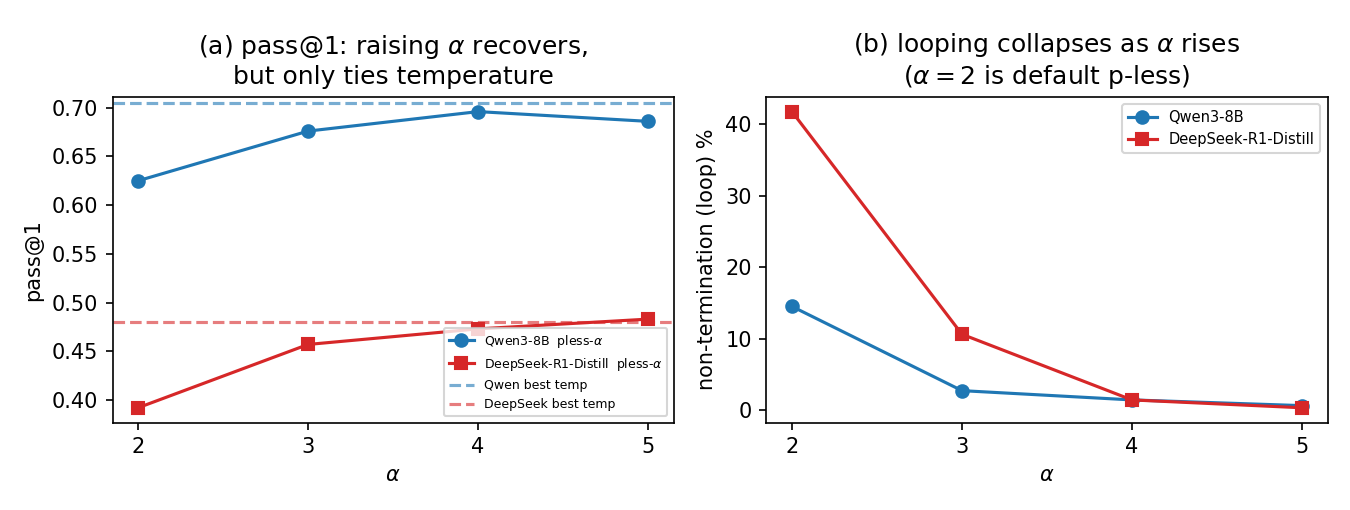
\includegraphics[width=\linewidth]{fig_apps_alpha.png}
\caption{APPS: (a) raising $\alpha$ recovers pass@1 but only ties the best temperature configuration
(dashed); (b) non-termination (looping) collapses as $\alpha$ rises from the $\alpha{=}2$ default.}
\label{fig:appsalpha}
\end{figure}

\paragraph{The honest punchline.} The best $\alpha$ setting only \emph{ties} well-tuned temperature:
DeepSeek $\alpha{=}5$ ($0.483$) $\approx$ temperature ($0.480$); on Qwen3 temperature ($0.705$)
\emph{beats} the best $\alpha$ ($0.686$). $\alpha$ is therefore a diagnostic lens and a repair for a
broken default, not a new state-of-the-art sampler.

\paragraph{Relation to the origin paper's R\'enyi form.} \citet{tan2025pless} (App.\ B.5) propose a
different generalization, $G_k=\exp(-H_k)=(\tsum_i p_i^k)^{1/(k-1)}$, but run no experiments at
$k\neq2$. Our raw power-sum $\tau_\alpha$ and their rooted $G_k$ coincide only at order 2 (both equal
the collision-entropy threshold); for order $>2$ they move in \emph{opposite directions}
(Table~\ref{tab:nonequiv}): $\tau_\alpha$ decreases (loosens, admits more tail tokens) while $G_k$
increases toward $\max_i p_i$ (tightens toward the mode). On $p{=}[0.45,0.25,0.15,0.10,0.05]$, sweeping
the order $2\!\to\!8$, $\tau_\alpha$ admits progressively more tokens (mode-only up to full support,
five distinct filters) while $G_k$ stays locked on the mode at every order---so no reparameterization
aligns their admitted sets, and the two are non-equivalent for order $>2$. We therefore describe our
sweep as an \emph{$\alpha$-frequency-moment} thresholding family and claim only the first
\emph{empirical} study of $\alpha>2$, not the idea of a R\'enyi generalization.

\begin{table}[t]\centering
\caption{The two R\'enyi forms on $p{=}[0.7,0.2,0.1]$: coincide at order 2, diverge in opposite
directions after. Computed value; see \texttt{paperA\_renyi\_nonequivalence.md}.}
\label{tab:nonequiv}
\begin{tabular}{cccc}
\toprule
order & $\tau_\alpha$ (ours) & $G_k$ (origin) & \\
\midrule
2 & 0.5400 & 0.5400 & (coincide) \\
3 & 0.3520 & 0.5933 & \\
4 & 0.2418 & 0.6230 & \\
5 & 0.1684 & 0.6406 & ($\to \max_i p_i{=}0.70$) \\
\bottomrule
\end{tabular}
\end{table}

\section{Prevention vs.\ rescue}\label{sec:prevention}
If a broken default ($\alpha=2$) loops, is it better to prevent the loop by choosing a flatter sampler
up front, or to detect and rescue it? We compare prevention (run $\alpha{=}5$ from the start) against a
reactive rescue (run $\alpha{=}2$, detect the loop with an $n$-gram monitor, chop back to onset, and
continue at $\alpha{=}5$). Prevention wins on the high-loop model (DeepSeek $0.483$ vs.\ adaptive
$0.457$) and ties on the low-loop model (Qwen $0.686$ vs.\ $0.682$; adaptive edges pass@10, $0.845$
vs.\ $0.833$)---the more a model loops, the more prevention beats surgical rescue. The
mechanistic reason is that $\alpha{=}5$'s flatter survivor set suppresses re-entry into the loop after
a chop, where $\alpha{=}2$ re-enters. Both, however, are matched by good temperature (Table~\ref{tab:apps}),
consistent with \S\ref{sec:alpha}: the lever matters only if one is committed to the p-less family.

\section{A reproducibility post-mortem}\label{sec:repro}
Getting these comparisons right required removing three silent bugs, each of which shifted pass@1
enough to change conclusions. (i) A transformers-v5 tokenizer routing bug (HF \#45488) fed the
DeepSeek model whitespace-mangled prompts (\texttt{def f(a, b):}\,$\to$\,\texttt{deff(a,b):}) under one
backend, depressing pass@1 by up to 22\,pp. (ii) A blanket uniform-smoothing guard added to prevent a
numerical crash silently perturbed the published p-less filter on \emph{every} step. (iii) A
float32 reduction over a large vocabulary could round the threshold above $\max_i p_i$ and prune every
token, yielding a NaN crash. Before fixing (i)--(ii), an ostensible ``adaptive $\gg$ prevention''
result appeared; after fixing them and putting all conditions on one backend, the ordering reversed to
the prevention$\ge$adaptive result reported above. We document the fixes and the corrected comparison
so that future decoding-method studies on reasoning models can avoid the same traps.

\section{Discussion and Limitations}\label{sec:discussion}
\paragraph{Where p-less helps / breaks.} On flat distributions (weak base models; instruct models at
$T\!\in\![0.6,1.0]$) p-less reproduces greedy's pass@1 with small non-zero diversity at zero
hyperparameter cost, and tops the \citet{shi2024decoding} panel on Llama-2-7B. On peaked distributions
(strong instruct models under diversity demand; long CoT) the threshold collapses to the mode:
pass@10 is dominated by temperature, and reasoning traces loop.

\paragraph{Limitations.} (i) p-less never \emph{beats} well-tuned temperature in our tests; its value
is the removed knob, not accuracy. (ii) We do not claim $\alpha$ is uniquely principled: the diversity
monotonicity we observe empirically also holds for top-$p$ and top-$k$, so $\alpha$ is one member of a
broader class, not a singularly-justified choice. We make no theoretical optimality claim. (iii) The
reasoning-model study covers two 8B models and one benchmark (APPS); (iv) 10 samples/task; bootstrap
CIs are deferred. (v) Cross-survey comparisons cross independent evaluation pipelines (a 4\,pp
temperature@0.7 pipeline gap is documented).

\paragraph{Practical recommendation.} For a code model of unknown peakedness, start with p-less at
$T{=}1.0$ and compare pass@1 to greedy on a small calibration set; if they match, keep p-less for its
calibration-free property; if pass@1 is materially worse, or if the model produces long chain-of-thought,
fall back to temperature in $[0.7,1.0]$ or raise $\alpha$ to escape the peakedness trap.

\section{Conclusion}\label{sec:conclusion}
p-less is a competitive but not dominant code-generation sampler whose behavior is governed by
distribution peakedness: a high-accuracy/low-diversity default that helps where distributions are flat
and silently breaks---collapsing to greedy and looping---where they are peaked. The R\'enyi-$\alpha$
family both diagnoses and repairs the failure but does not beat well-tuned temperature. The most
transferable lesson may be methodological: parameter-free does not mean assumption-free, and small
tokenizer- or numerics-level bugs can fabricate decoding-method effects larger than the effects under
study.

\bibliographystyle{plainnat}
\bibliography{refs}

\appendix
\section{Additional tables and figures}
\td{Move here: full APPS decoder tables (12/15 configs) from
docs/decoder\_comparison\_cot\_apps\_\{deepseek,qwen3\}.md; the $T_1/T_2$ decomposition
(draft.md \S4.4); per-model MBPP/HE headline table (draft.md Table 2); structural-diversity bars
(Fig.); detector configuration and the majorization brute-force note.}

\end{document}
